\documentclass[a4j]{jarticle}
\usepackage{listings}
\usepackage{color}
\usepackage[dvipdfmx]{graphicx}
\definecolor{OliveGreen}{rgb}{0.0,0.6,0.0}
\lstset{
  basicstyle={\ttfamily},
  identifierstyle={\small},
  commentstyle={\smallitshape \color[rgb]{0,0.5,0}},
  keywordstyle={\small\bfseries},
  ndkeywordstyle={\small},
  stringstyle={\small\ttfamily},
  frame={tb},
  breaklines=true,
  columns=[l]{fullflexible},
  numbers=left,
  xrightmargin=0zw,
  xleftmargin=0zw,
  numberstyle={\scriptsize},
  stepnumber=1,
  numbersep=1zw,
  lineskip=-0.5ex,
  linewidth=15cm
}

\begin{document}

{\rm \huge 課題}
  \section{課題1}
    \subsection{ 10 進数を 16 進数に変える javascript プログラム}
      参照\\
      ex110short.html\\
      1\_1.png
    \subsection{16 進数の掛け算表を表示する javascript プログラム}
      参照\\
      1\_2.png\\
      ex120.html
  \section{課題2}
    \subsection{ボタンを押すたびに拝啓が変化する javascript プログラム}
      参照\\
      ex210short.html\\
      2\_1.png
    \subsection{行の追加削除を行う javascript プログラム}
        参照\\
      2\_2.png\\
      ex220.html
  \section{課題3}
    別ファイル提出
  \section{課題4}
    \subsection{4.1 jQuery で書かれたコードの省略}
      参照\\
      ex410short.html\\
      4\_1.png
    \subsection{外部 API を呼び出すプログラム}
      参照\\
      4\_2.png\\
      ex421long.html
    \subsection{アニメーションを表示するプログラム}
      参照\\
      4\_3.png\\
      ex430.html
  \section{課題5}
    \subsection{自分で考えたサイトのフォーム}
      \subsubsection{どのような web サイトを想定したか}
        あるカフェでの注文をネットから受ける際の web フォームを想定する。
        まず、店頭で商品を受け取る際に必要な名前を入力する欄を一番初めに設置する。続け
        て商品を選ぶリストとそれに伴ってドリンクの氷の量や甘さ、タピオカなどのトッピ
        ングに関しての量や有無を確認する欄を設ける。最後に注文に関して個人的な要望が
        あれば記載できるように備考欄を付け加える。
      \subsubsection{構築した(1)の仕様を満たすウェブページ}
        参照\\
        ex510dev.html
      \subsubsection{スマホやタブレットでは操作性がどのように変化するか。}
        スマホで実験結果を確認すると、自動でスマホの画面の大きさに変化し全体的に縦
        長な配置となった。例えばもともと名前や甘さなど選択対象を指定する見出しはリス
        トやラジオボタンと並んで配置されていたが、スマホで閲覧した際は見出し、リストの
        ように順番になって縦に伸びた配置になっていた。操作に関してはクリックがなくな
        りすべて指のタッチで行えるようになったため操作性が上がったように感じる。特に
        シークバーなどは自分の指でつかんでいるような感覚であった。さらに画面を下にス
        クロールする際は、マウスなどで動かすのではなく指でフォームの余白をなぞること
        で画面のスクロールをすることができた。\\
        参照\\
        5\_1\_3.png
      \subsubsection{テーマローラサイト用いた発展課題}
        参照\\
        5\_1\_4.png
    \subsection{PC およびスマホに対応するウェブサイト}
      \subsubsection{プログラム}
        参照\\
        5\_2\_1.png
      \subsubsection{PC とモバイル双方に対応する web サイトを構築する際に気を付けること}
            PC とモバイルデバイスでは画面のサイズが違うため両方に対応したサイトを作る
        ときには特にそこに注意しないといけない。PC 画面で作った横長のサイトだとスマホ
        で見るときには折り返しが多く見にくかったり、画面からははみ出たりして操作性や
        閲覧性に支障をきたす場合がある。一方でスマートフォンだけに対応したサイトだと、
        縦長なサイトになってしまいスクロールの回数が増え操作性に欠ける。さらに PC での
        操作だけを考えていると、ボタンが多く小さくなりがちだが、スマホサイトで表示した
        ときそういったボタンは操作性に問題が出てくるためスマホサイトにした場合でも指
        で操作できるような UI を心がけるべきである。
  \section{課題6}
    \subsection{javascript不正コード埋め込実験}
      \subsubsection{chrome と firefox で不正コードを実行したときの挙動}
        Firefox(旧)では不正コードが実行された。一方で chrome では実行されなかった\\
        参照\\
        6\_1\_1\_ff.png\\
        6\_1\_1\_ch.png
      \subsubsection{スマホで不正コードを実行したときの挙動}
        どちらも埋め込んだ不正コードは実行されなかった。おそらくブラウザ側で何らかの対策行われていのだと考えられる。\\
        参照\\
        6\_1\_2\_ff.jpg\\
        6\_1\_2\_ch.jpg
    \subsection{img の脆弱性をついた不正コード}
      http://192.168.2.139:8080/2ndWeek/ex620.html\#” \textgreater \textless img\ src =x 以降を示す\\
      (1) Javascript の機能を用いた\\
      onerror = console.log(document.getElementsByTagName(“table”))\textgreater \textless/img\textgreater\\
      (2) jQuery の機能を用いた\\
      onerror = console.log(\$(“table”))\textgreater \textless/img\textgreater \\
      を行うことでテーブルのデータを取り出すことができる。\\
      参照\\
      6\_2\_1.png\\
      6\_2\_2.png\\
      \vspace{2em}\\
      この実験で得た知識を用いて法律に接するような行為は行いません。
      \begin{flushright}
        金子泰之\qquad 2019 年 11 月 11 日
      \end{flushright}
    \subsection{課題自体廃止}
    \subsection{DOM basef XSS に対して}
      まず初めに開発者は、作成したコードに対し外部から不正な入力が入る可能性があること知らないといけない。その上で、ソースからのデータを出力する際に、\textless script\textgreater に含まれる特殊記号が文字ではなく実行開始命令として解釈されることで不正な入力が起こるため、特殊な記号を文字列に変換することで無害化する必要がある。この無害化を行うことをエスケース処理やサニタイジング処理といい、jQueryではjQuery.parseHTML()などがある。また、ソースからのデータをHTMLとして処理すると不正コードが混在していた場合HTMLとして実行されてしまうことがあるので、テキストとして代入することで安全に出力することができる。さらに、あらゆる脆弱性をついた攻撃は日々進化するため、新たな脆弱性に対処できるように最新のバージョンのライブラリを用いる必要がある。セキュアコーディング手法は一般に公開されているため、セキュリティガイドラインに準拠してコーディングを行うべきであるがこれはまだ容易でないため、作成したコードをこのガイドラインに準拠した形に自動的に変換するソフトウェアの開発が研究されている。これが実現すればコード作成者はセキュリティーの知識が乏しくともセキュリティガイドラインに準拠したプログラムを自由に書くことが出来るようになる。そういった意味では日々進化する攻撃手法をプログラマーはすべて知る必要がなくなるので負担が減ると考えられる。また、プログラマーの教育に関して作成したコードを仮想環境で実行し、あらゆる脆弱性をついて耐えられることが出来るか調べられる環境などがあればプログラマーがそれぞれの脆弱性に対して対処できると思うし、セキュリティガイドラインの内容を実際に実装するような勉強会などがあればプログラマーのセキュリティリテラシーが向上すると考えられる。
      \vspace{1cm}
      \noindent

      出典:\\
      鈴木 富明、白井 丈晴、小林 真也、川端 秀明、西垣 正勝「セキュリティガイドラインに準拠したアプリケーション作成支援に関する一提案」

\newpage
{\rm \huge ソースコード}
  \lstinputlisting[caption = ex110.html]{../webapp/1stWeek/ex110.html}
  \newpage
  \lstinputlisting[caption = ex120.html]{../webapp/1stWeek/ex120.html}
  \newpage
  \lstinputlisting[caption = ex210.html]{../webapp/1stWeek/ex210.html}
  \newpage
  \lstinputlisting[caption = ex220.html]{../webapp/1stWeek/ex220.html}
  \newpage
  \lstinputlisting[caption =ex410short.html ]{../webapp/2ndWeek/ex410short.html}
  \newpage
  \lstinputlisting[caption =ex421long.html ]{../webapp/2ndWeek/ex421long.html}
  \newpage
  \lstinputlisting[caption = ex430.html]{../webapp/2ndWeek/ex430.html}
  \newpage
  \lstinputlisting[caption = ex510dev.html]{../webapp/2ndWeek/ex510dev.html}
  \newpage
  \lstinputlisting[caption = ex520\_and\_521.html]{../webapp/2ndWeek/ex520_and_521.html}
  \newpage

\newpage
{\rm \huge 画像}

  \begin{figure}[htbp]
    \centering
    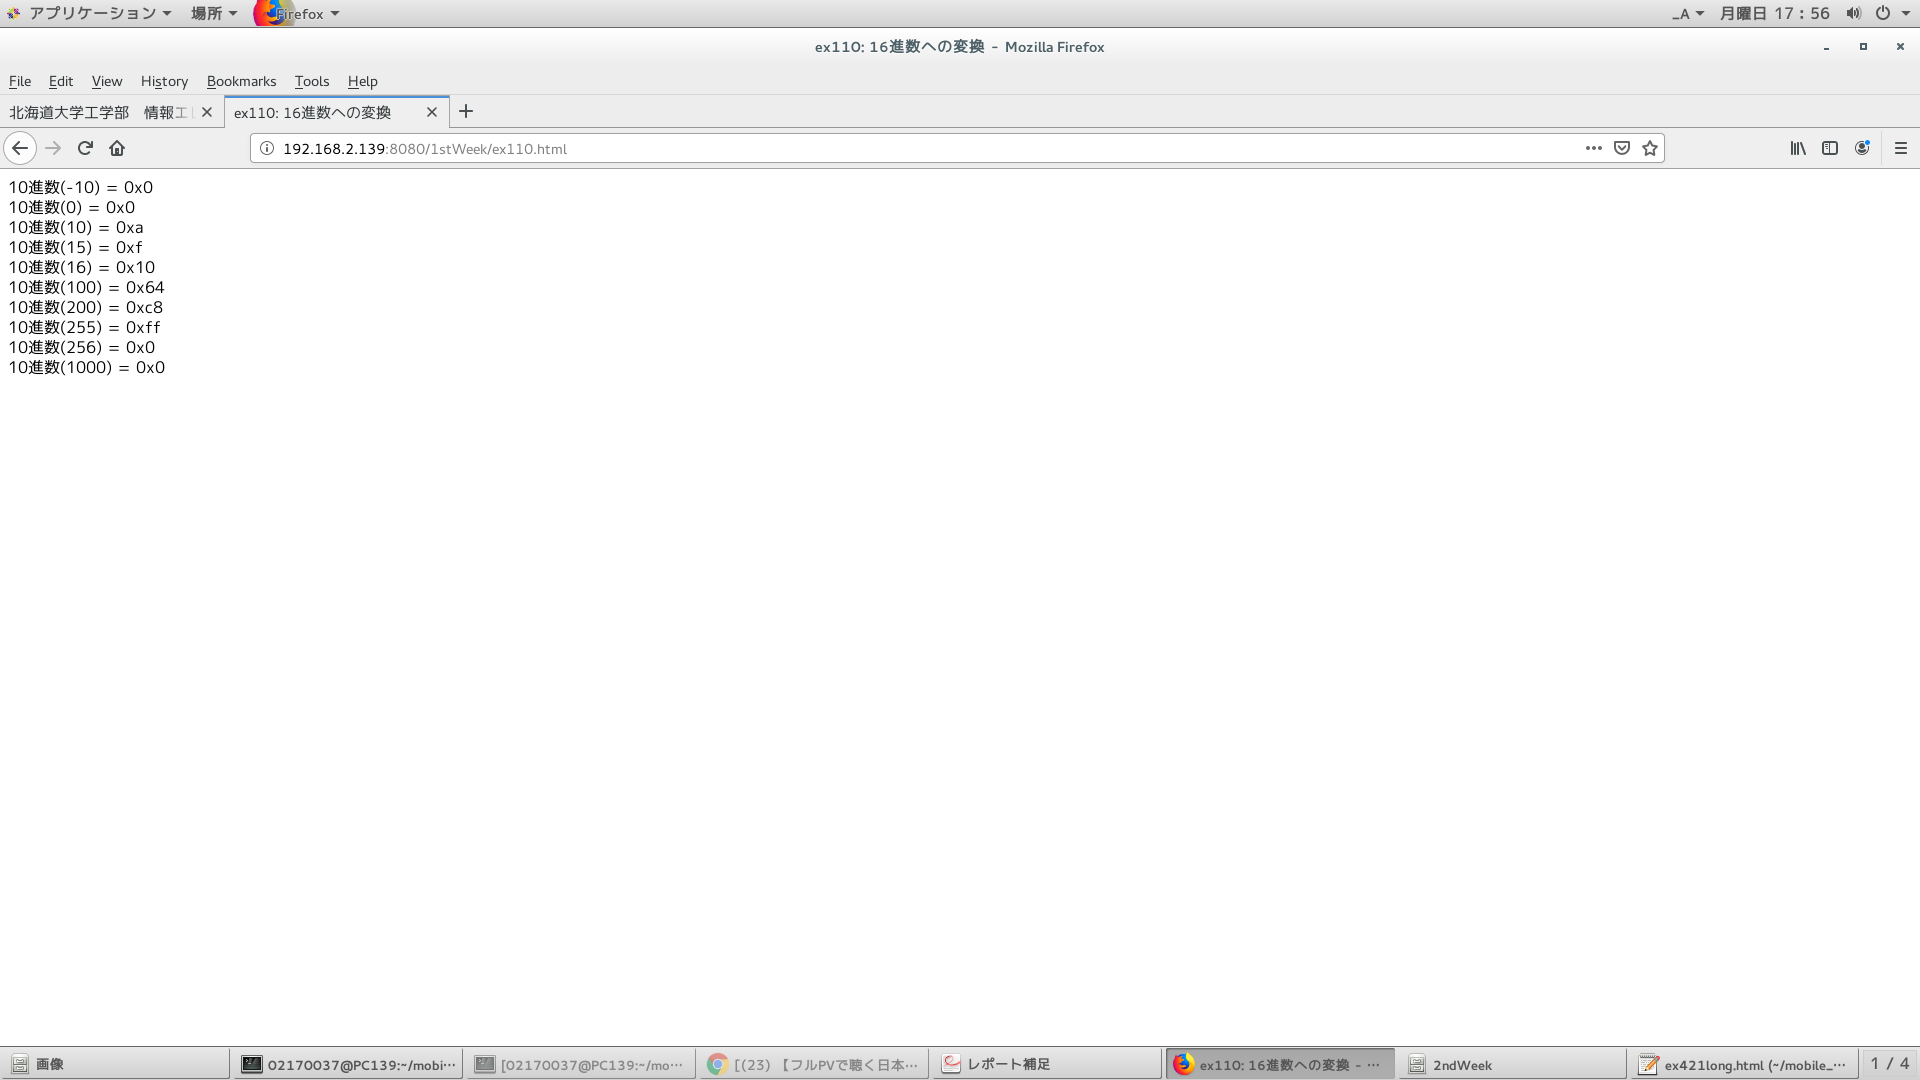
\includegraphics[width=13cm]{../webapp/png/1_1.png}
    \caption{1\_1.png}
  \end{figure}

  \vspace{1cm}
  \begin{figure}[htbp]
    \centering
    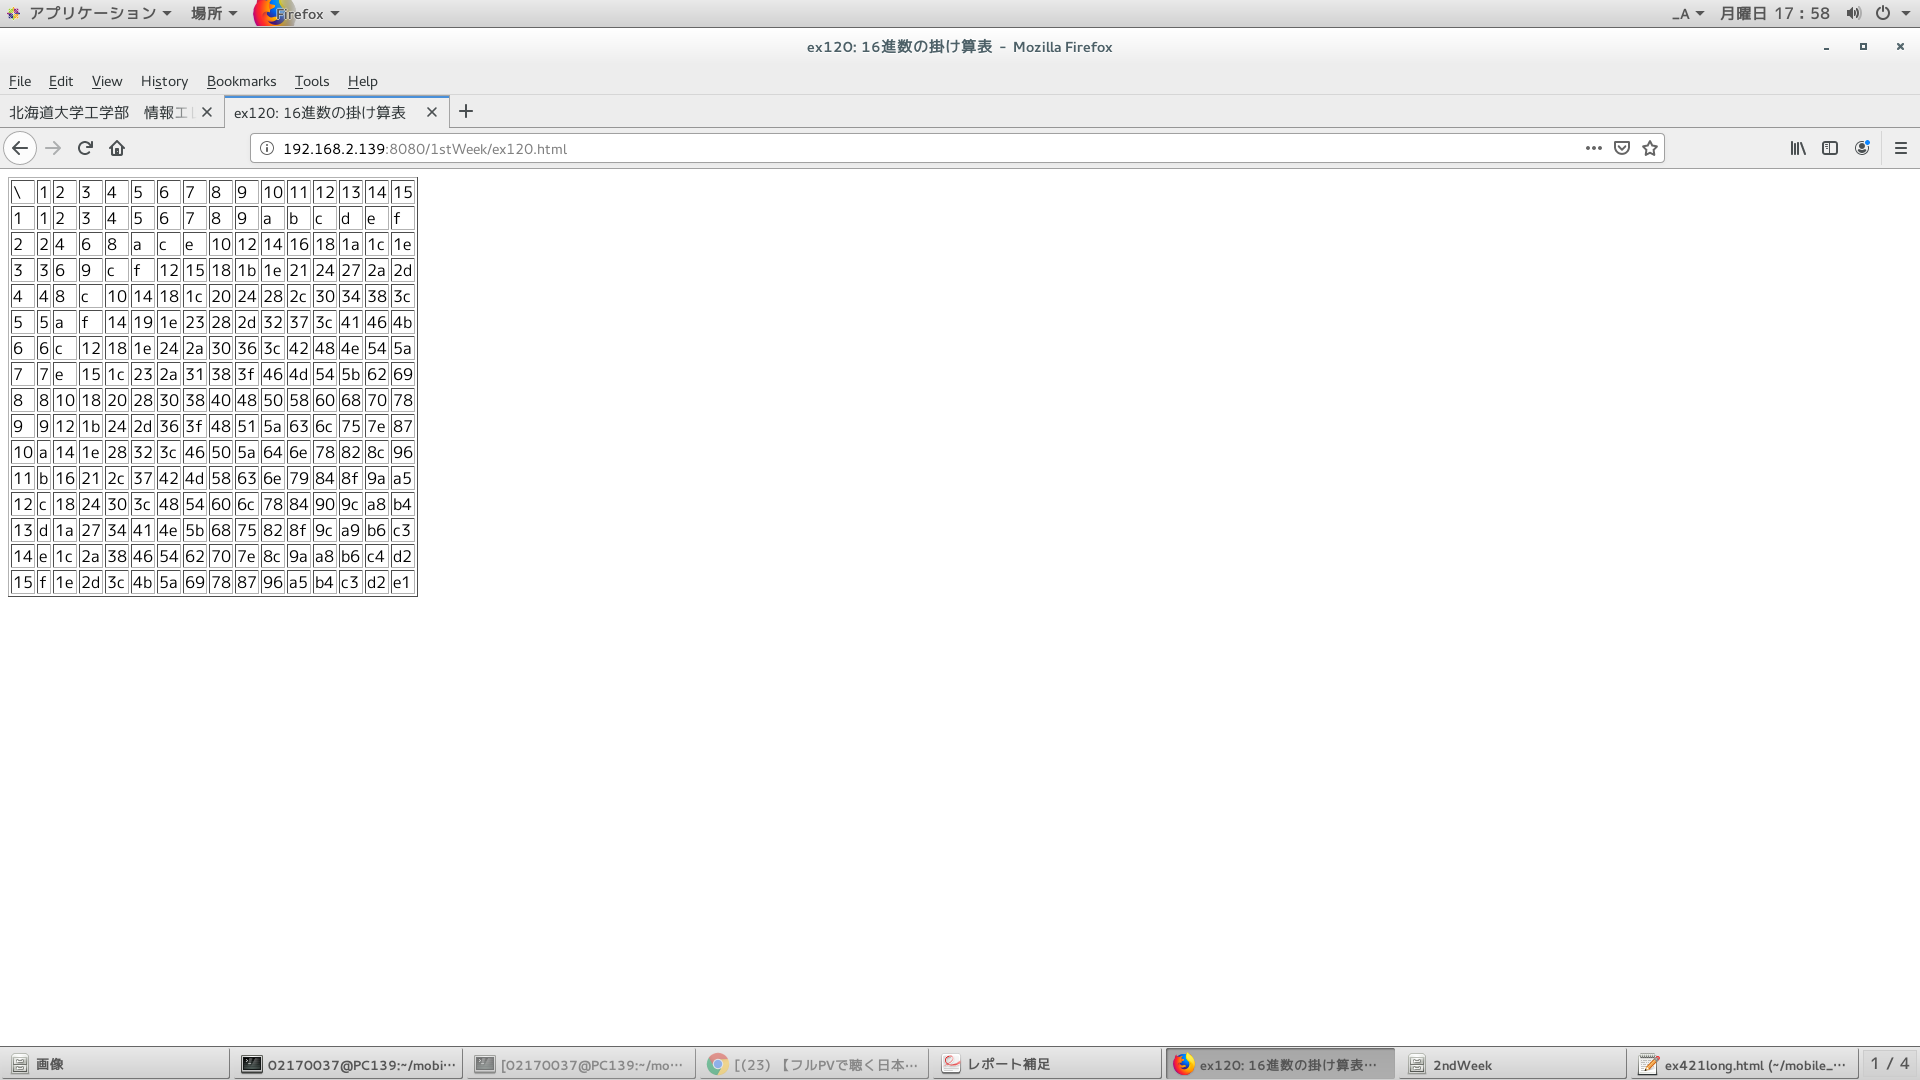
\includegraphics[width=13cm]{../webapp/png/1_2.png}
    \caption{1\_2.png}
  \end{figure}

  \vspace{1cm}
  \begin{figure}[htbp]
    \centering
    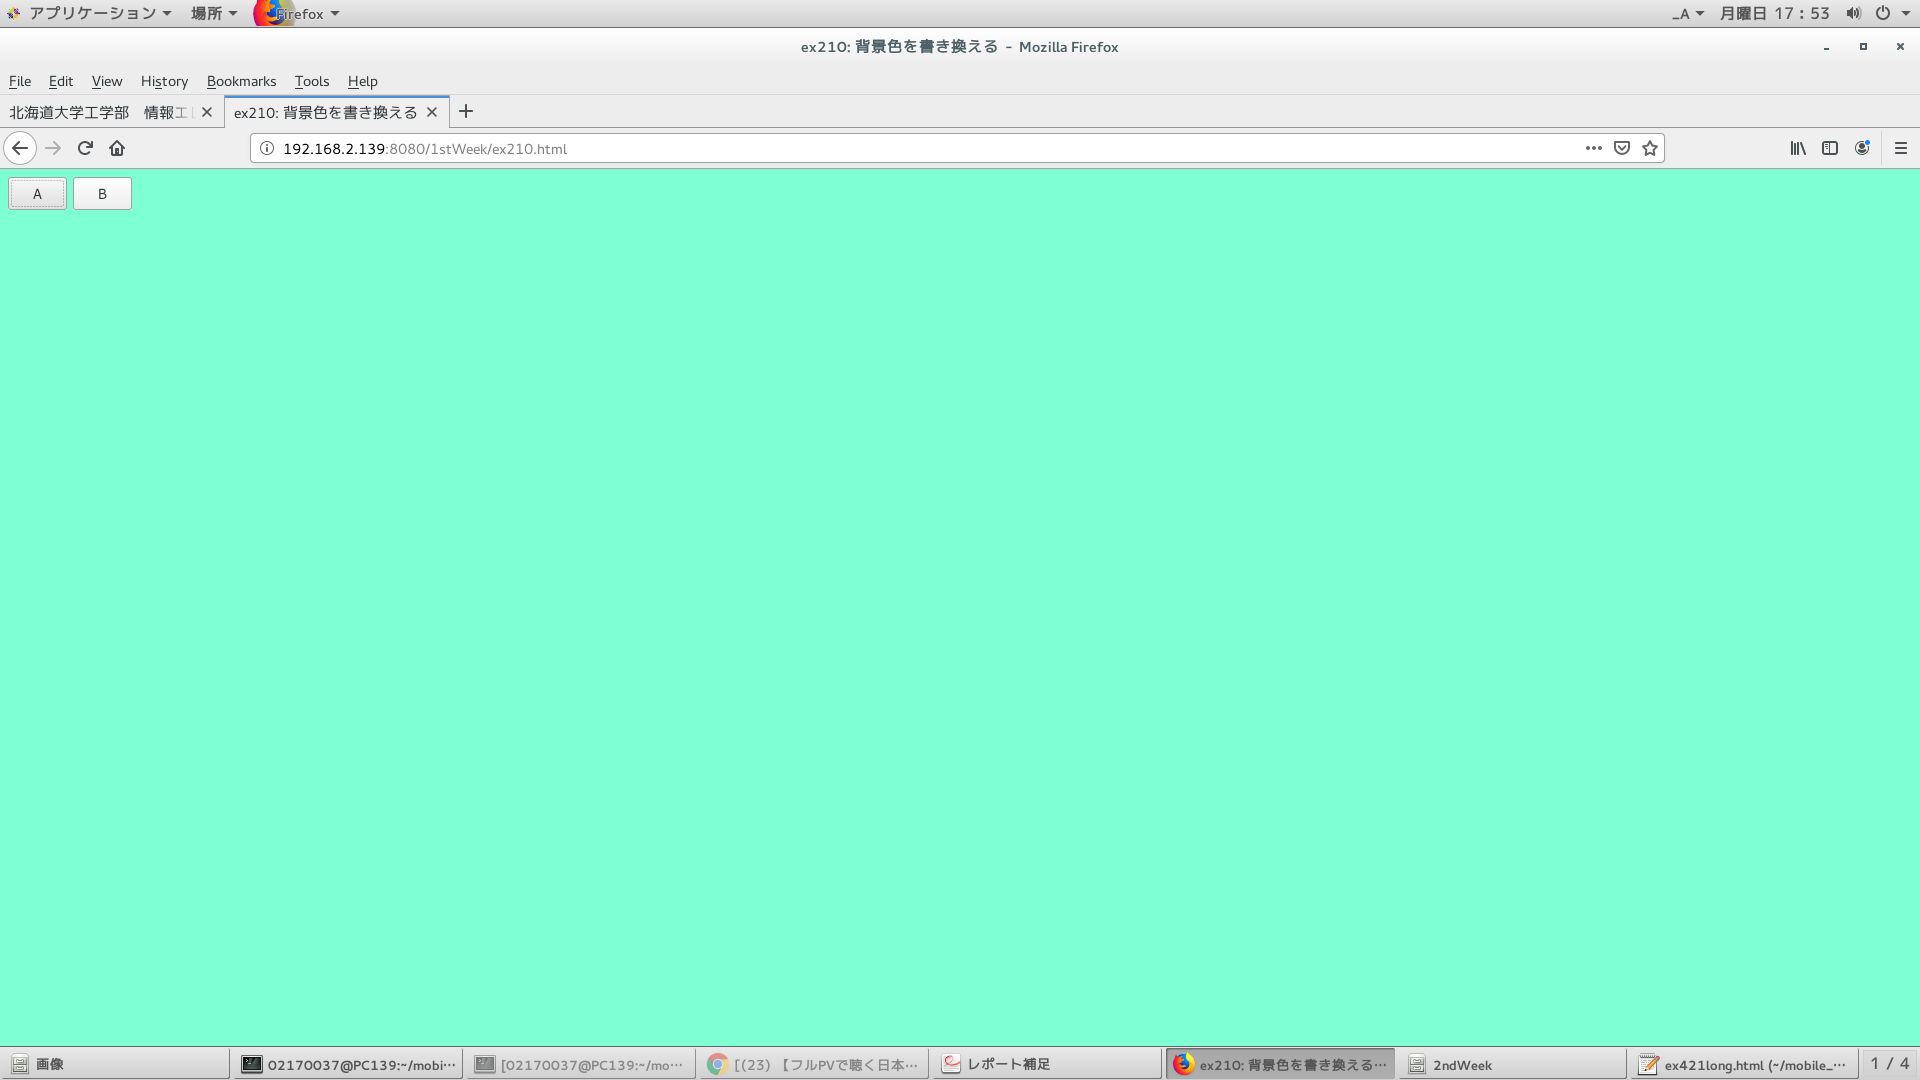
\includegraphics[width=13cm]{../webapp/png/2_1.png}
    \caption{2\_1.png}
  \end{figure}

  \vspace{1cm}
  \begin{figure}[htbp]
    \centering
    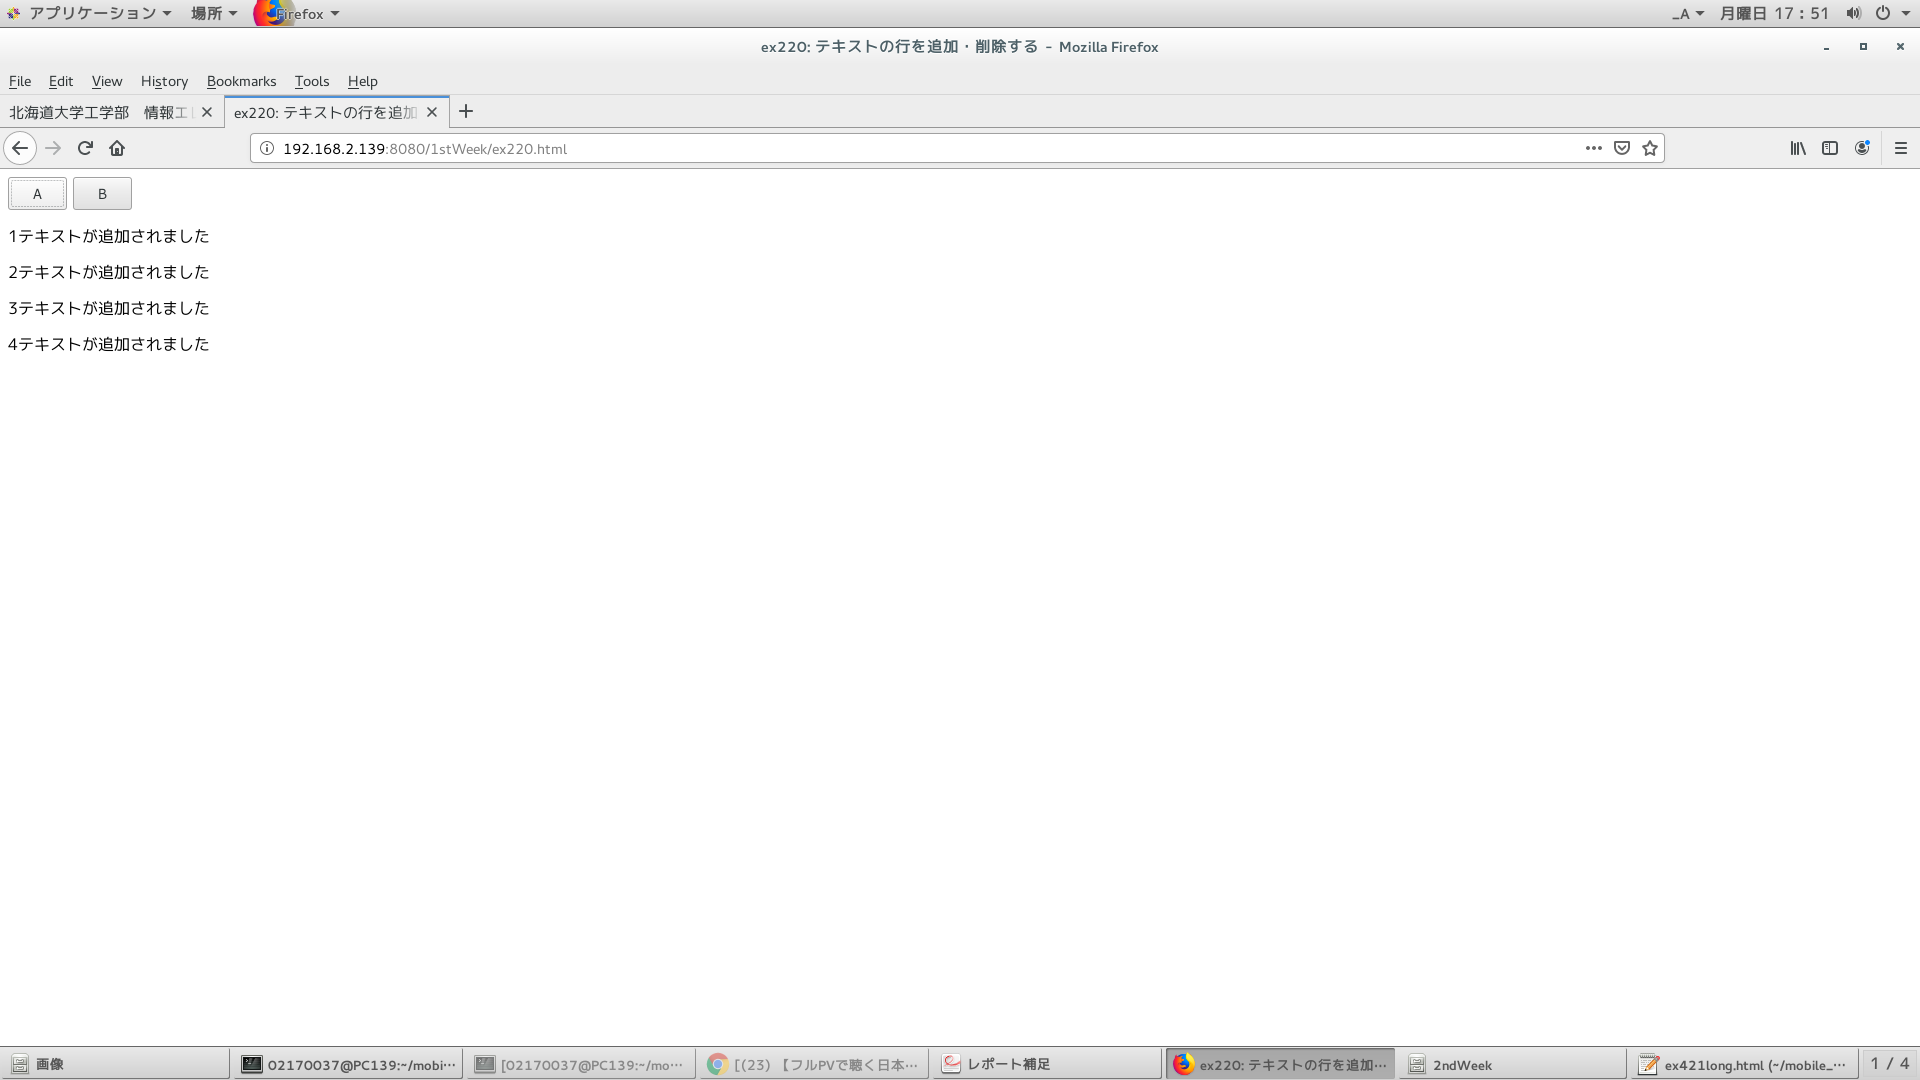
\includegraphics[width=13cm]{../webapp/png/2_2.png}
    \caption{2\_2.png}
  \end{figure}

  \vspace{1cm}
  \begin{figure}[htbp]
    \centering
    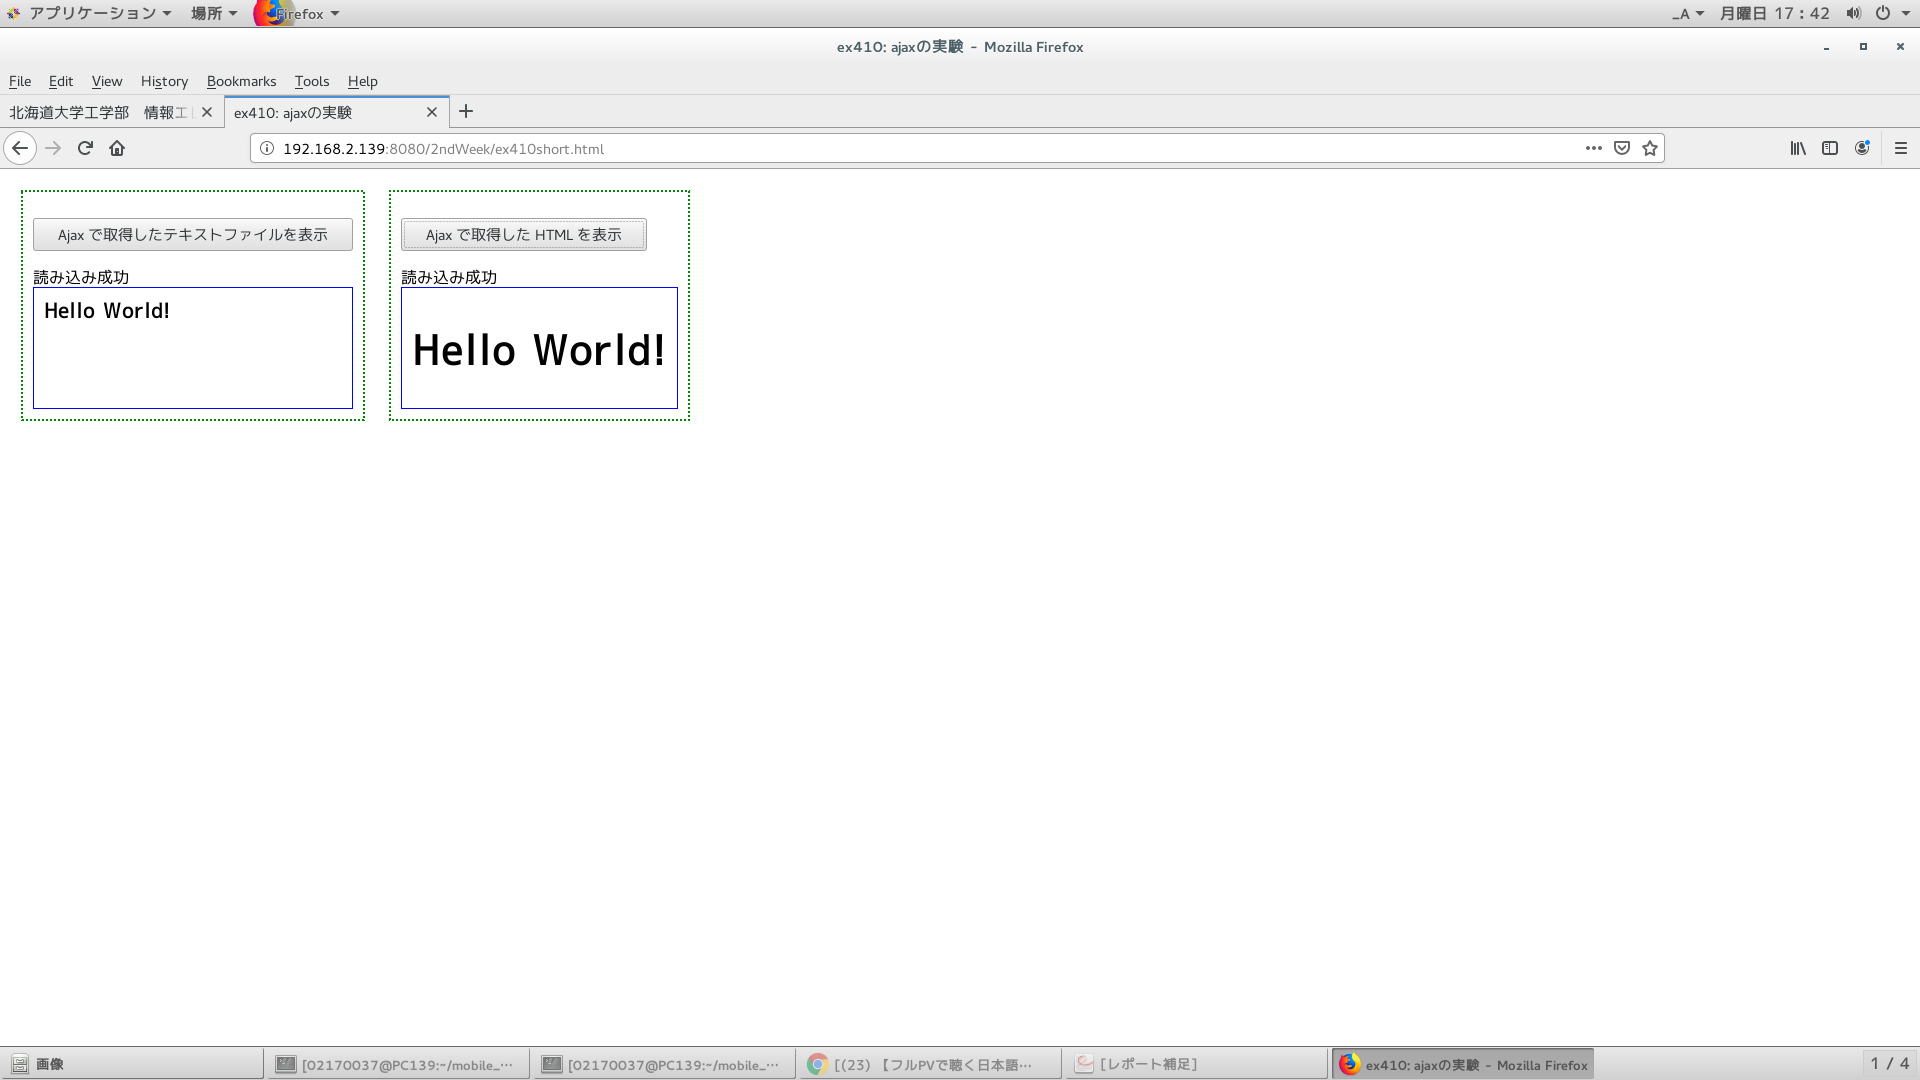
\includegraphics[width=13cm]{../webapp/png/4_1.png}
    \caption{4\_1.png}
  \end{figure}

  \vspace{1cm}
  \begin{figure}[htbp]
    \centering
    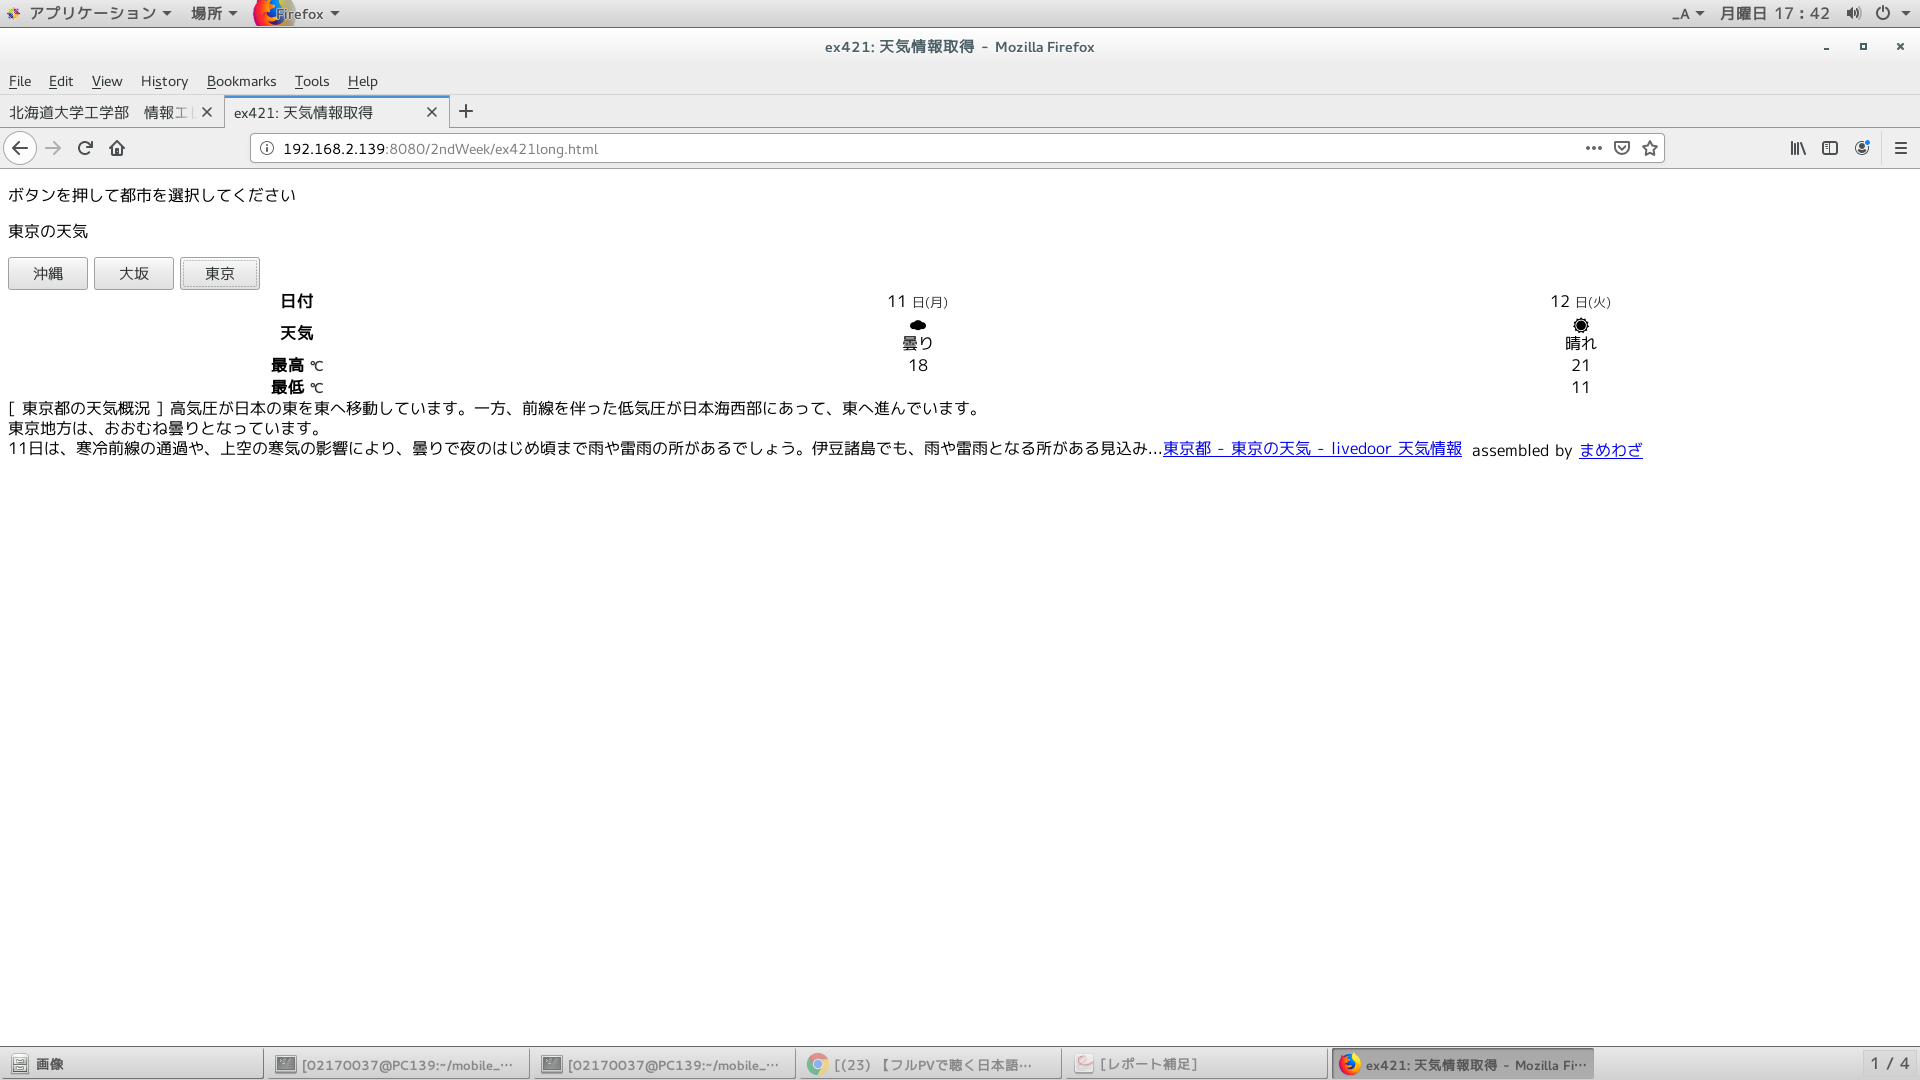
\includegraphics[width=13cm]{../webapp/png/4-2.png}
    \caption{4\_2.png}
  \end{figure}

  \vspace{1cm}
  \begin{figure}[htbp]
    \centering
    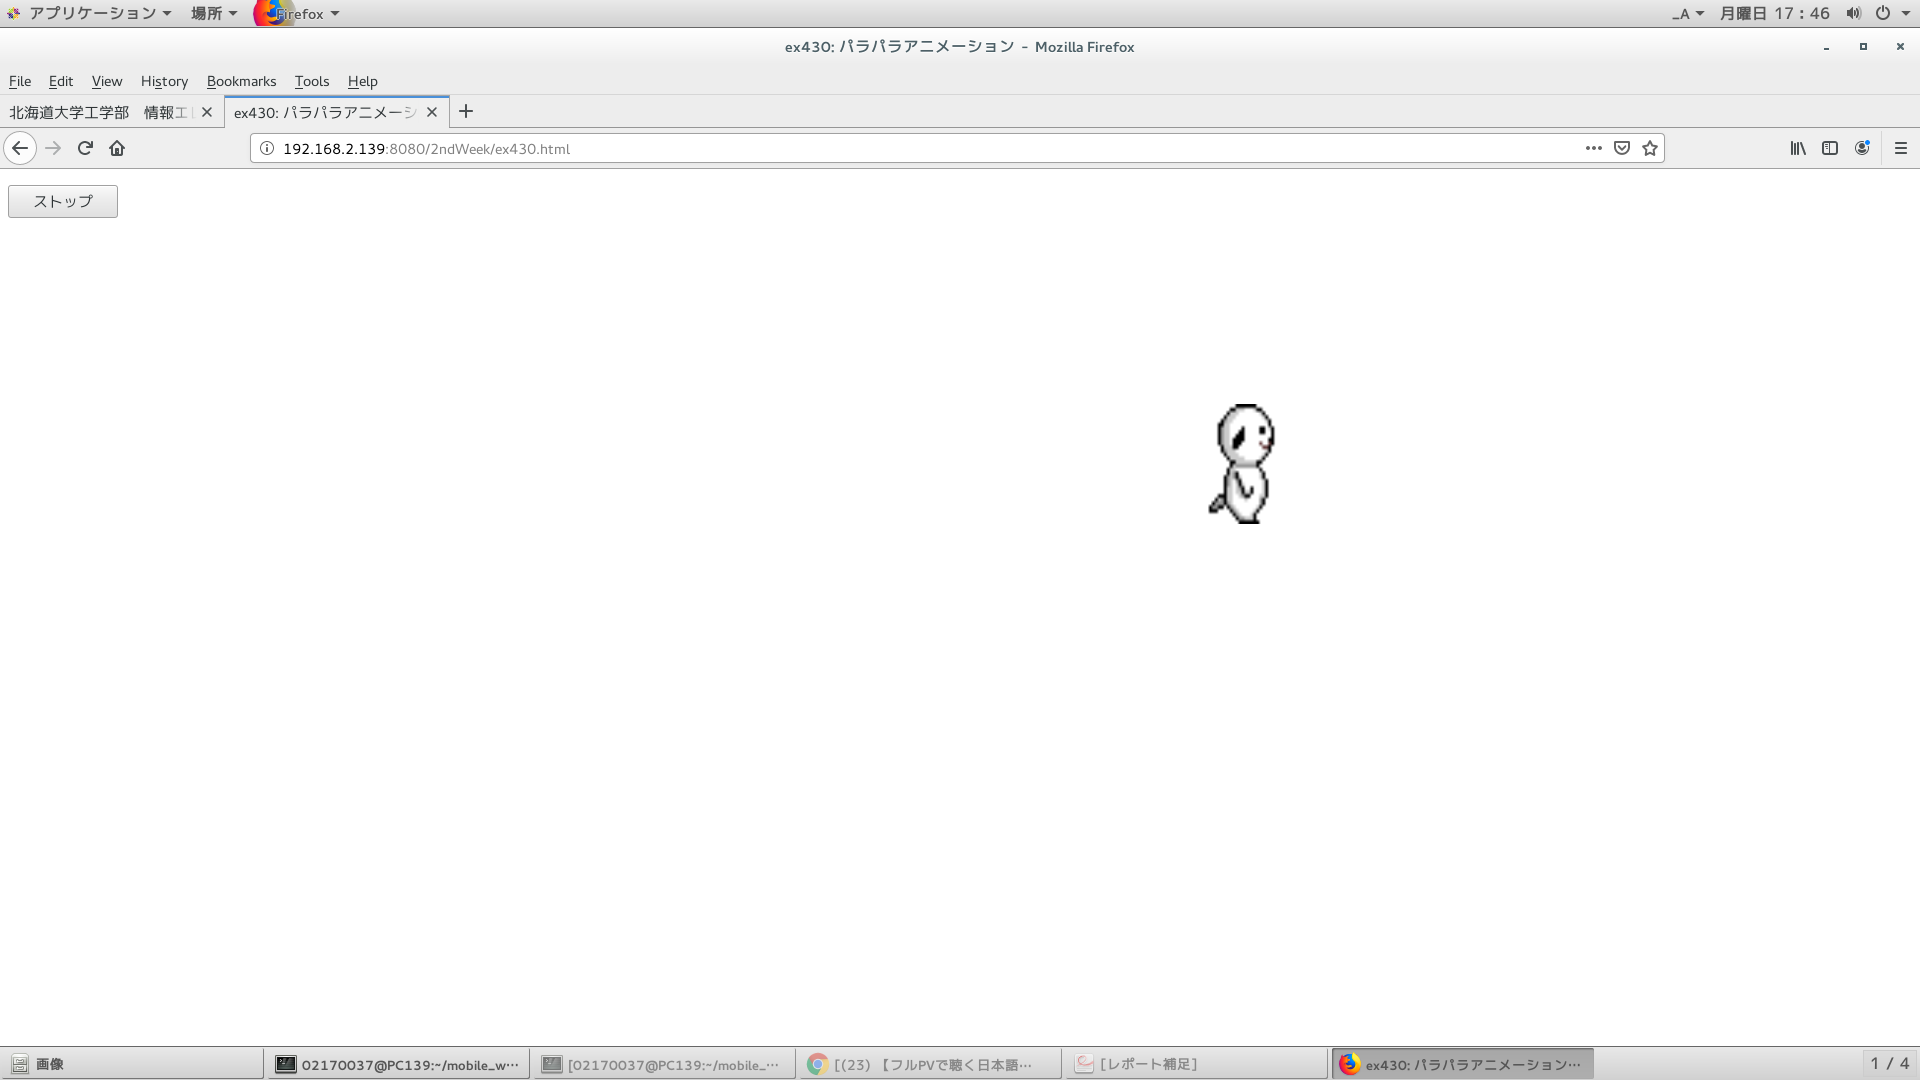
\includegraphics[width=13cm]{../webapp/png/4_3.png}
    \caption{4\_3.png}
  \end{figure}

  \vspace{1cm}
  \begin{figure}[htbp]
    \centering
    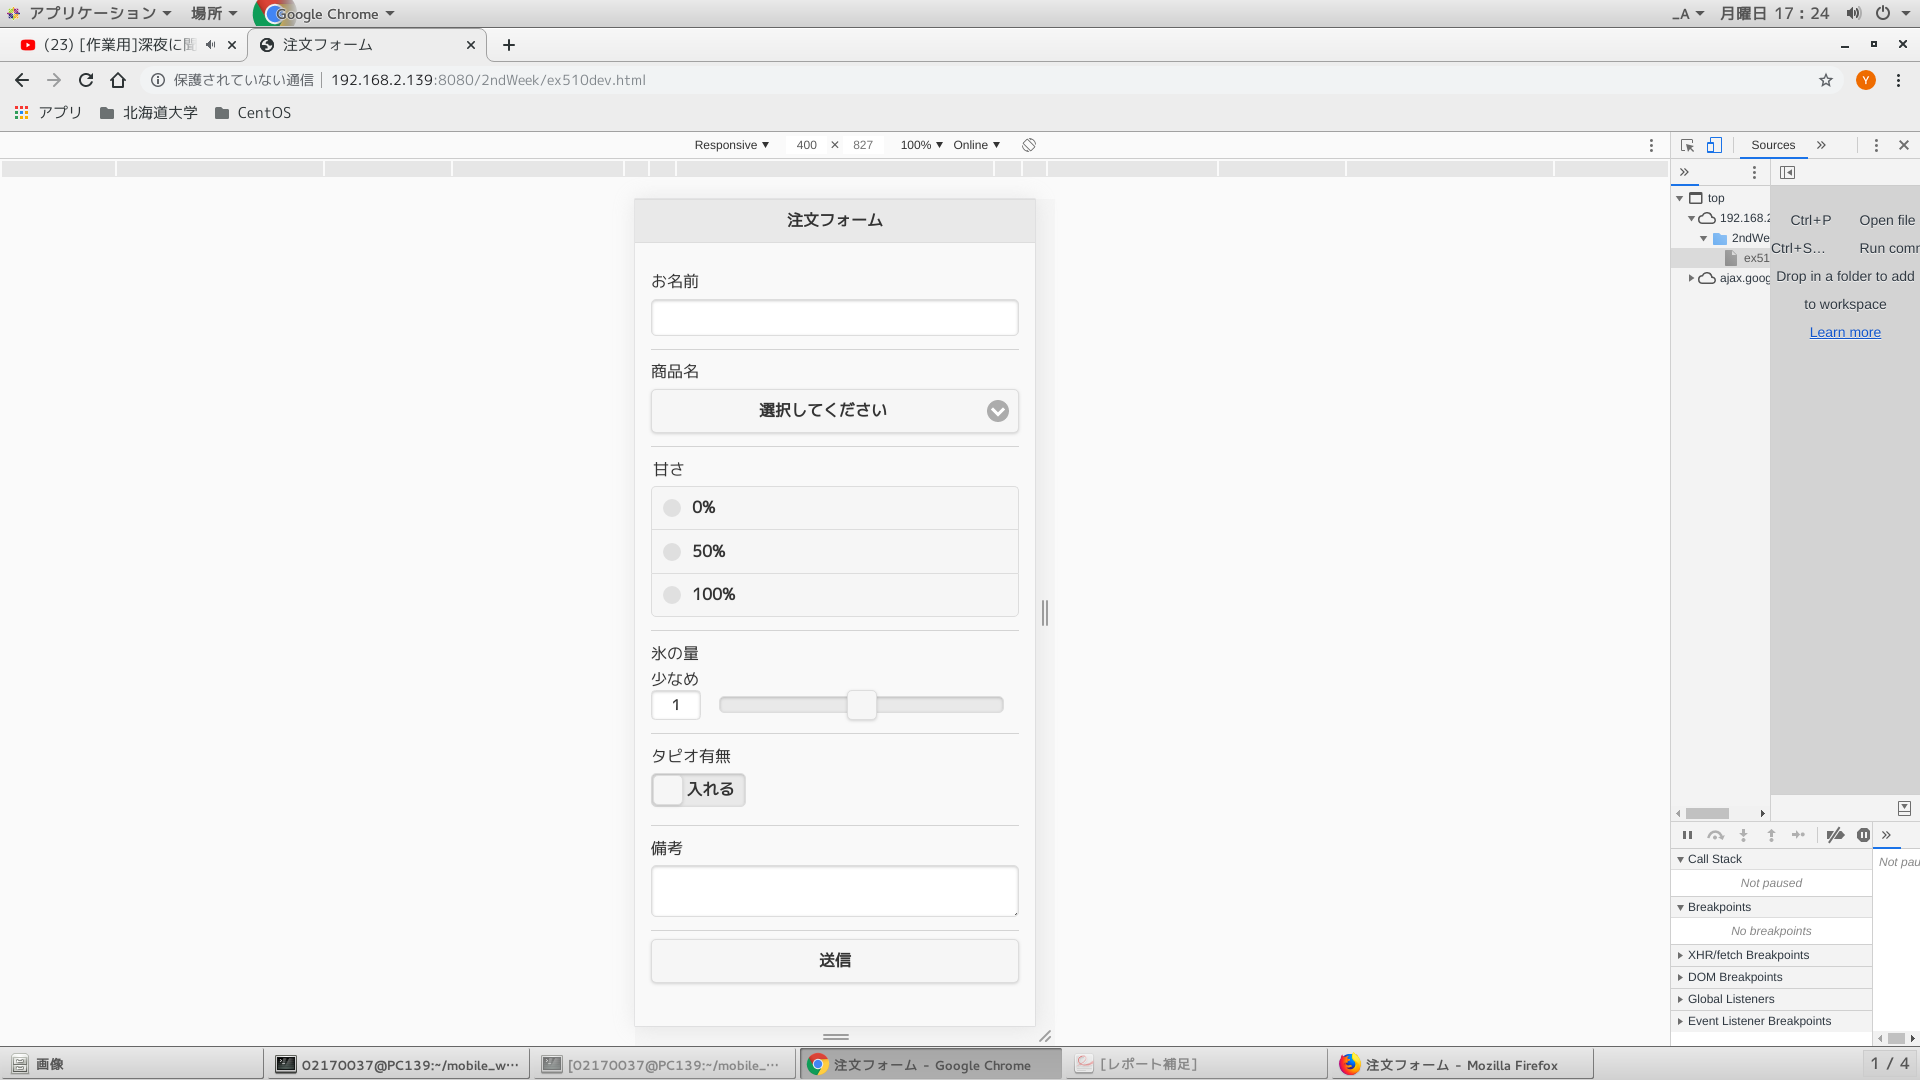
\includegraphics[width=13cm]{../webapp/png/5_1_3.png}
    \caption{5\_1\_3.png}
  \end{figure}

  \vspace{1cm}
  \begin{figure}[htbp]
    \centering
    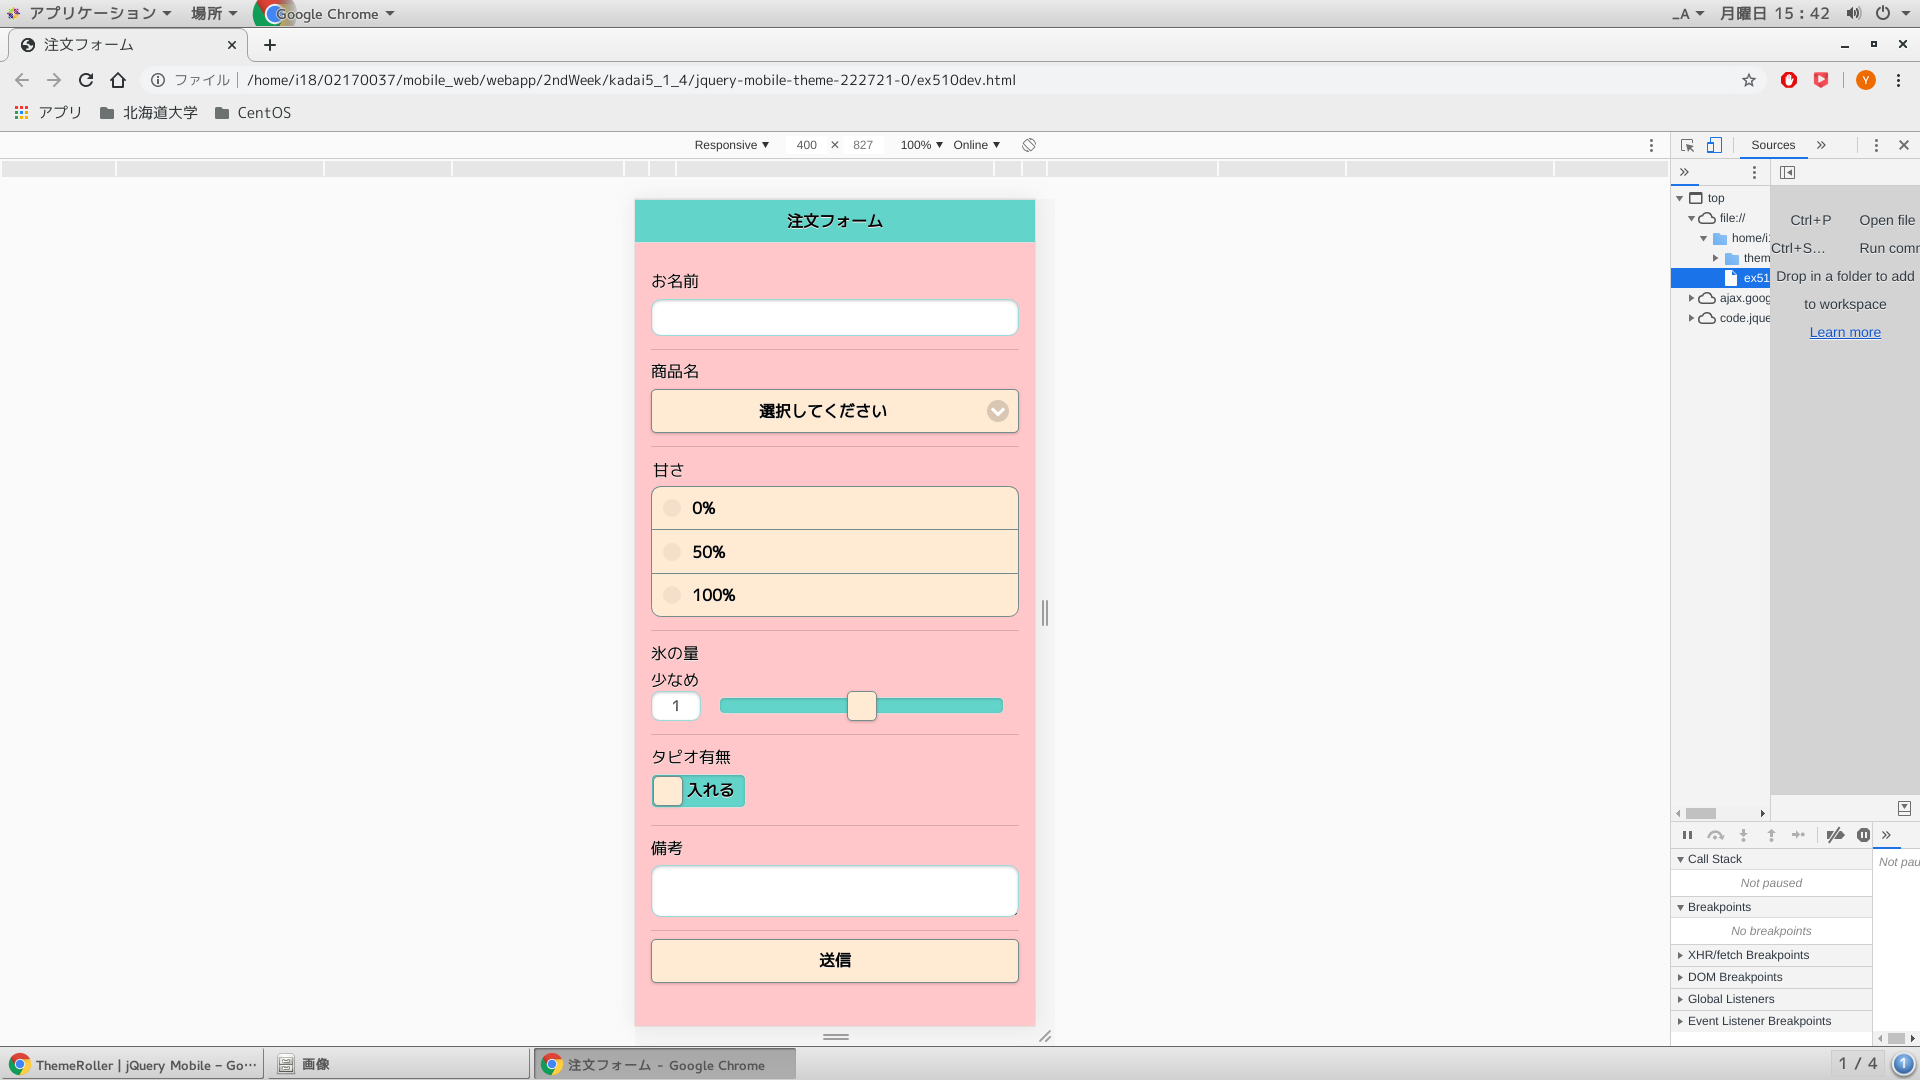
\includegraphics[width=13cm]{../webapp/png/5_1_4.png}
    \caption{5\_1\_4.png}
  \end{figure}

  \vspace{1cm}
  \begin{figure}[htbp]
    \centering
    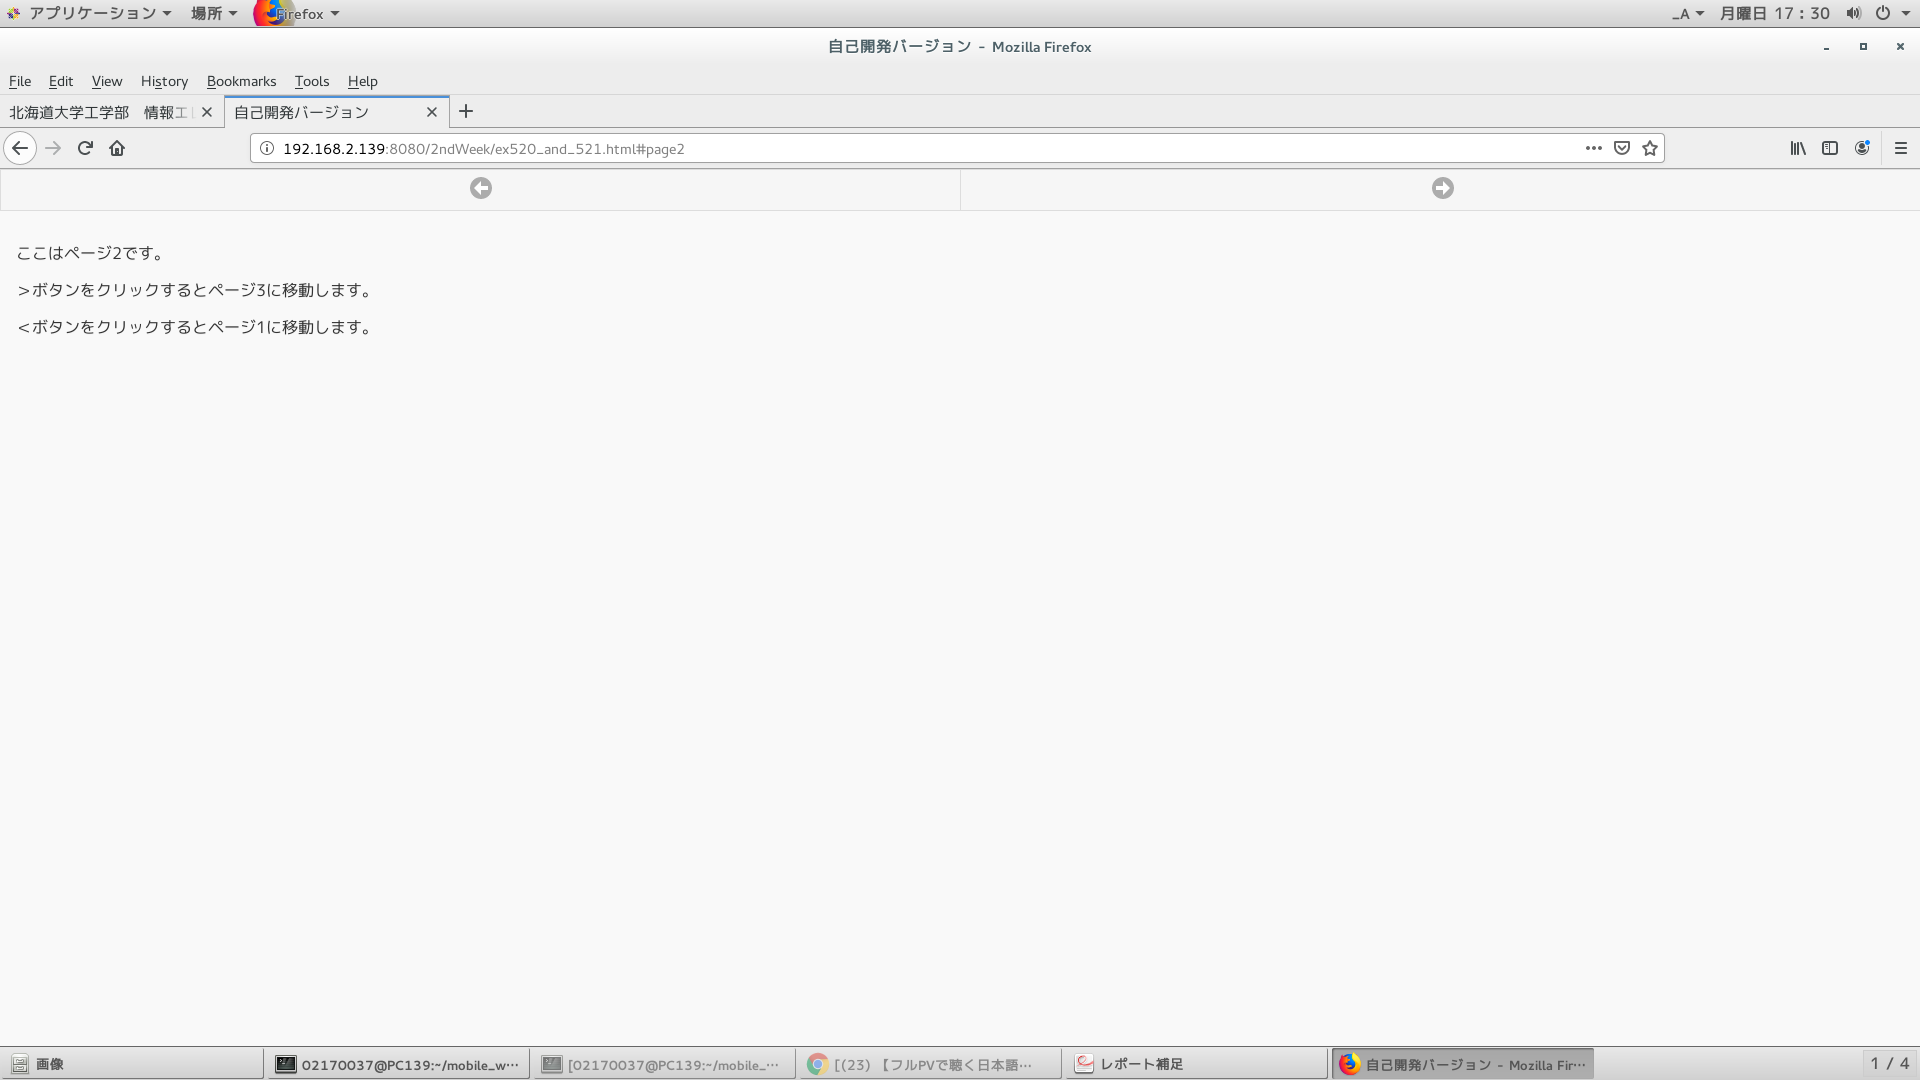
\includegraphics[width=13cm]{../webapp/png/5_2_1.png}
    \caption{5\_2\_1.png}
  \end{figure}

  \vspace{1cm}
  \begin{figure}[htbp]
    \centering
    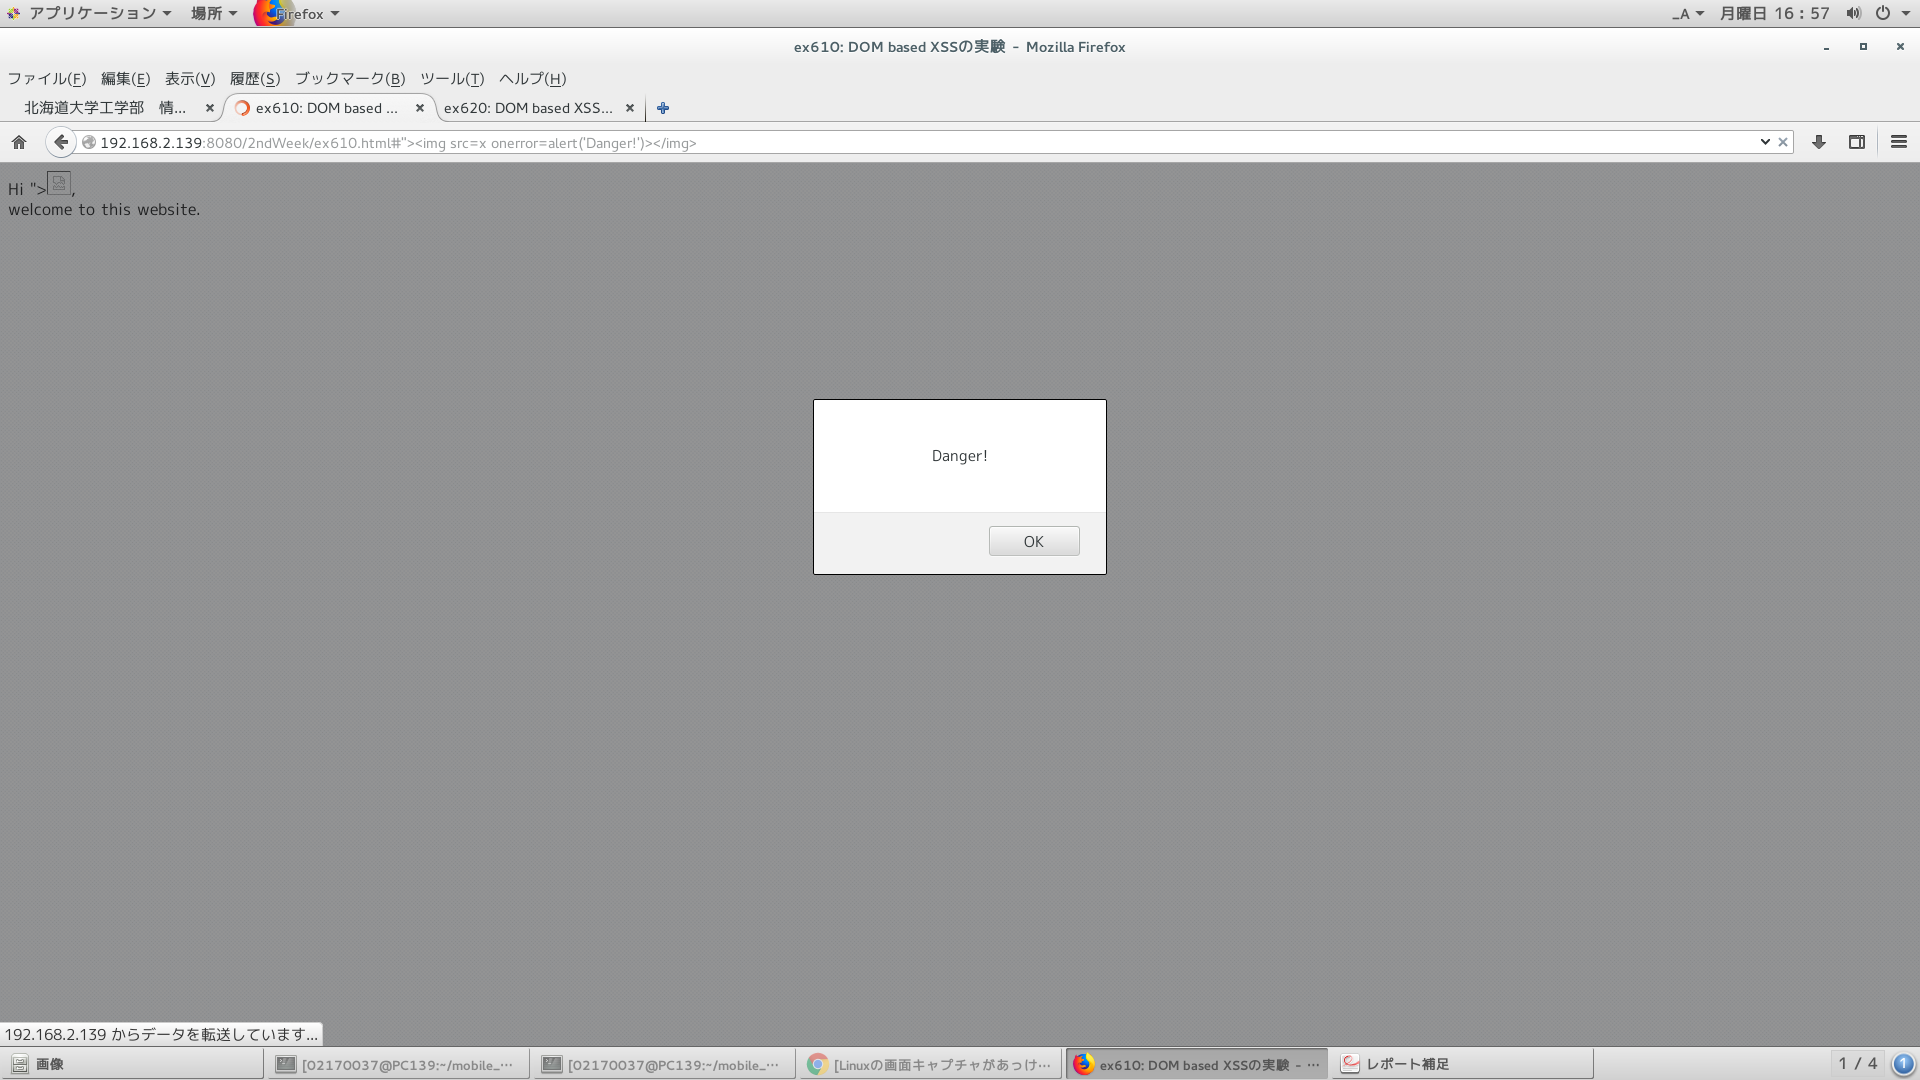
\includegraphics[width=13cm]{../webapp/png/6_1_1_ff.png}
    \caption{6\_1\_1\_ff.png}
  \end{figure}

  \vspace{1cm}
  \begin{figure}[htbp]
    \centering
    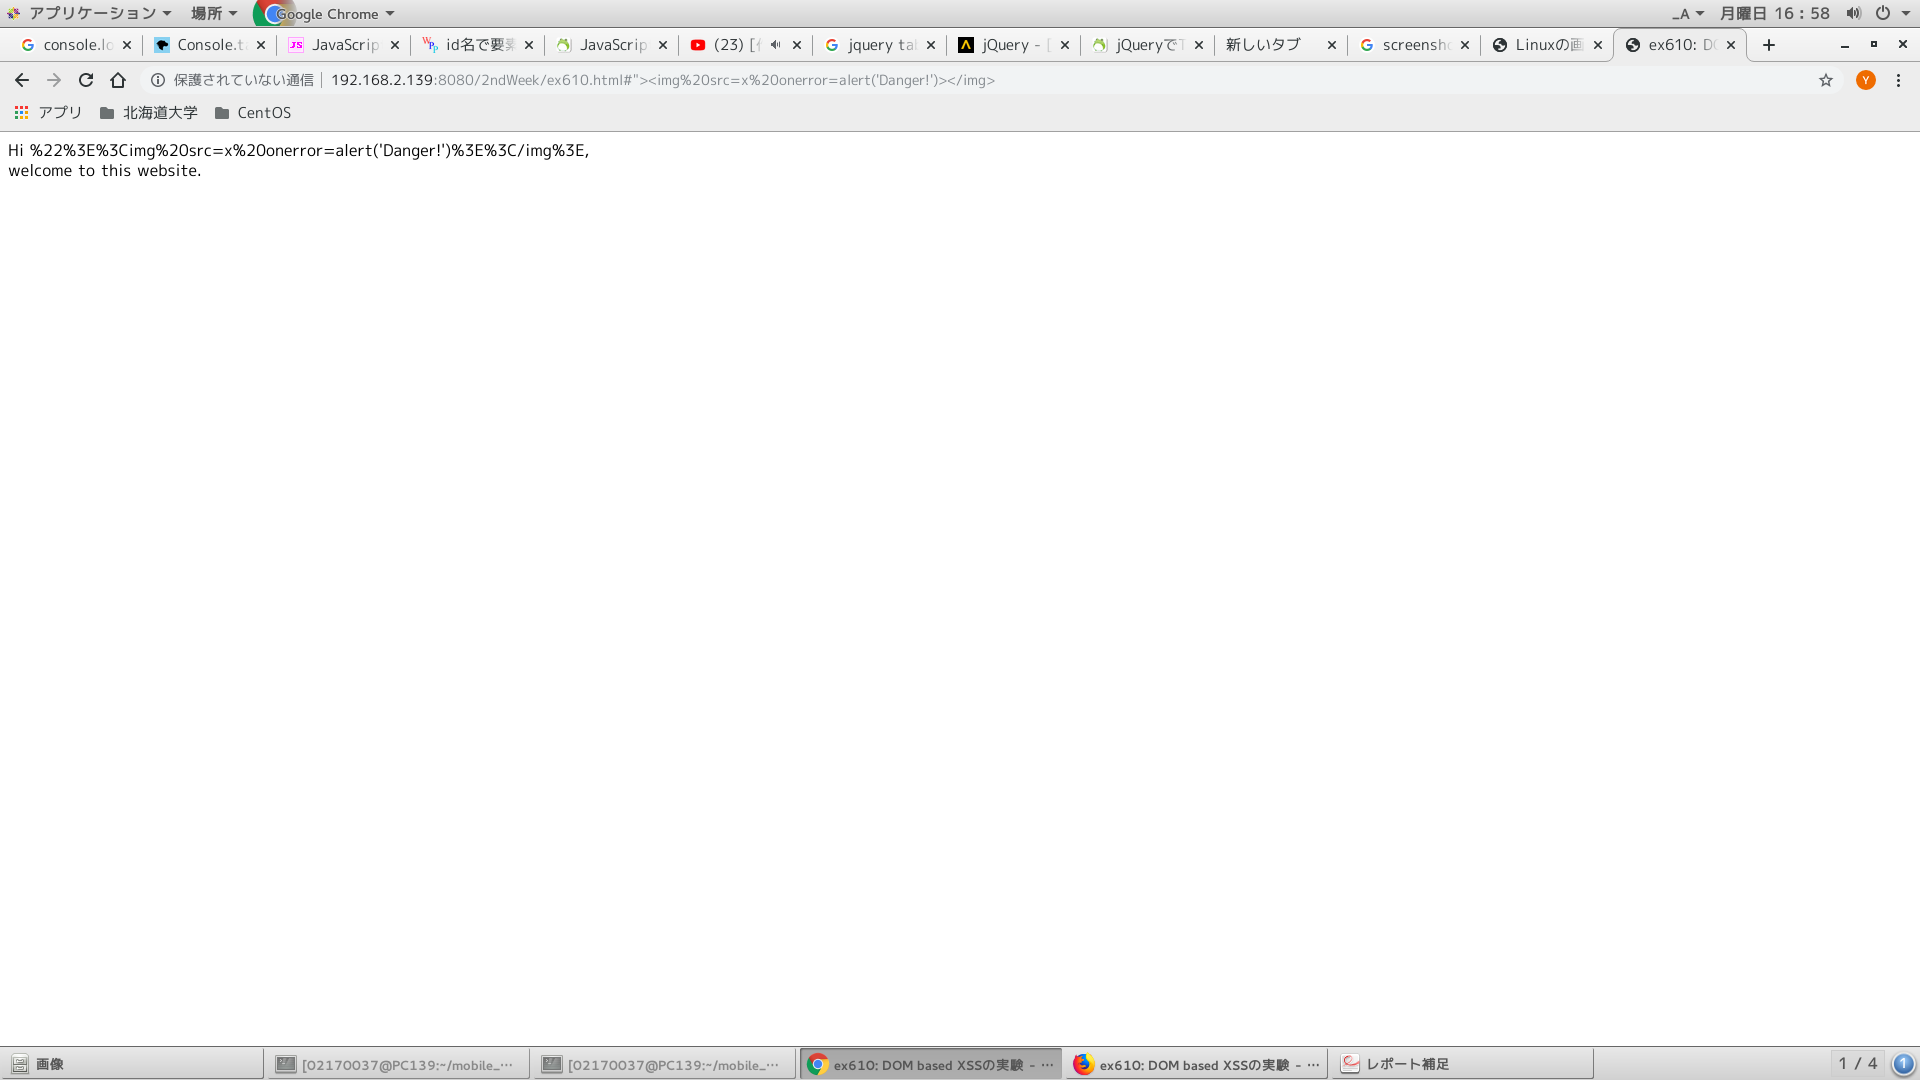
\includegraphics[width=13cm]{../webapp/png/6_1_1_ch.png}
    \caption{6\_1\_1\_ch.png}
  \end{figure}


  \vspace{1cm}
  \begin{figure}[htbp]
    \centering
    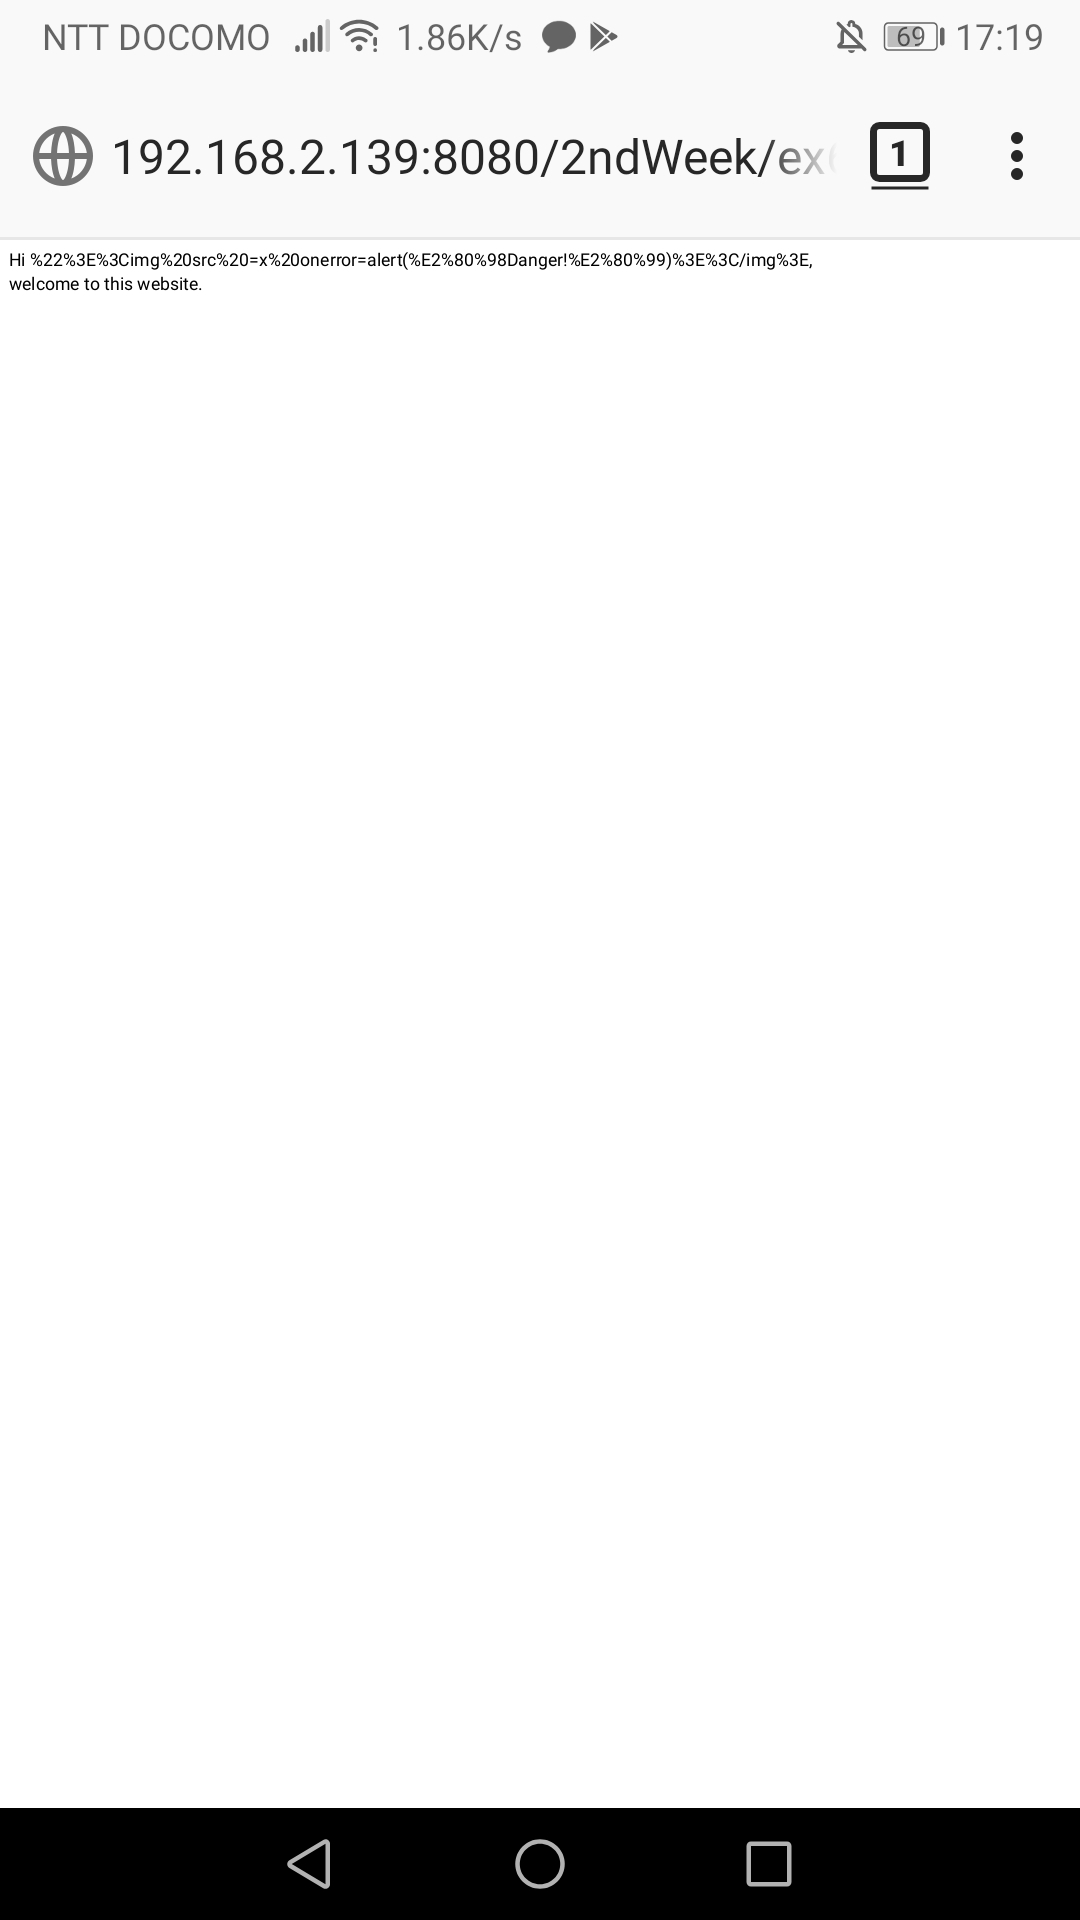
\includegraphics[width=10cm]{../webapp/png/6_1_2ff.jpg}
    \caption{6\_1\_2\_ff.jpg}
  \end{figure}


  \vspace{1cm}
  \begin{figure}[htbp]
    \centering
    
\includegraphics[width=10cm]{../webapp/png/6_1_2_ch.jpg}
    \caption{6\_1\_2\_ch.jpg}
  \end{figure}


  \vspace{1cm}
  \begin{figure}[htbp]
    \centering
    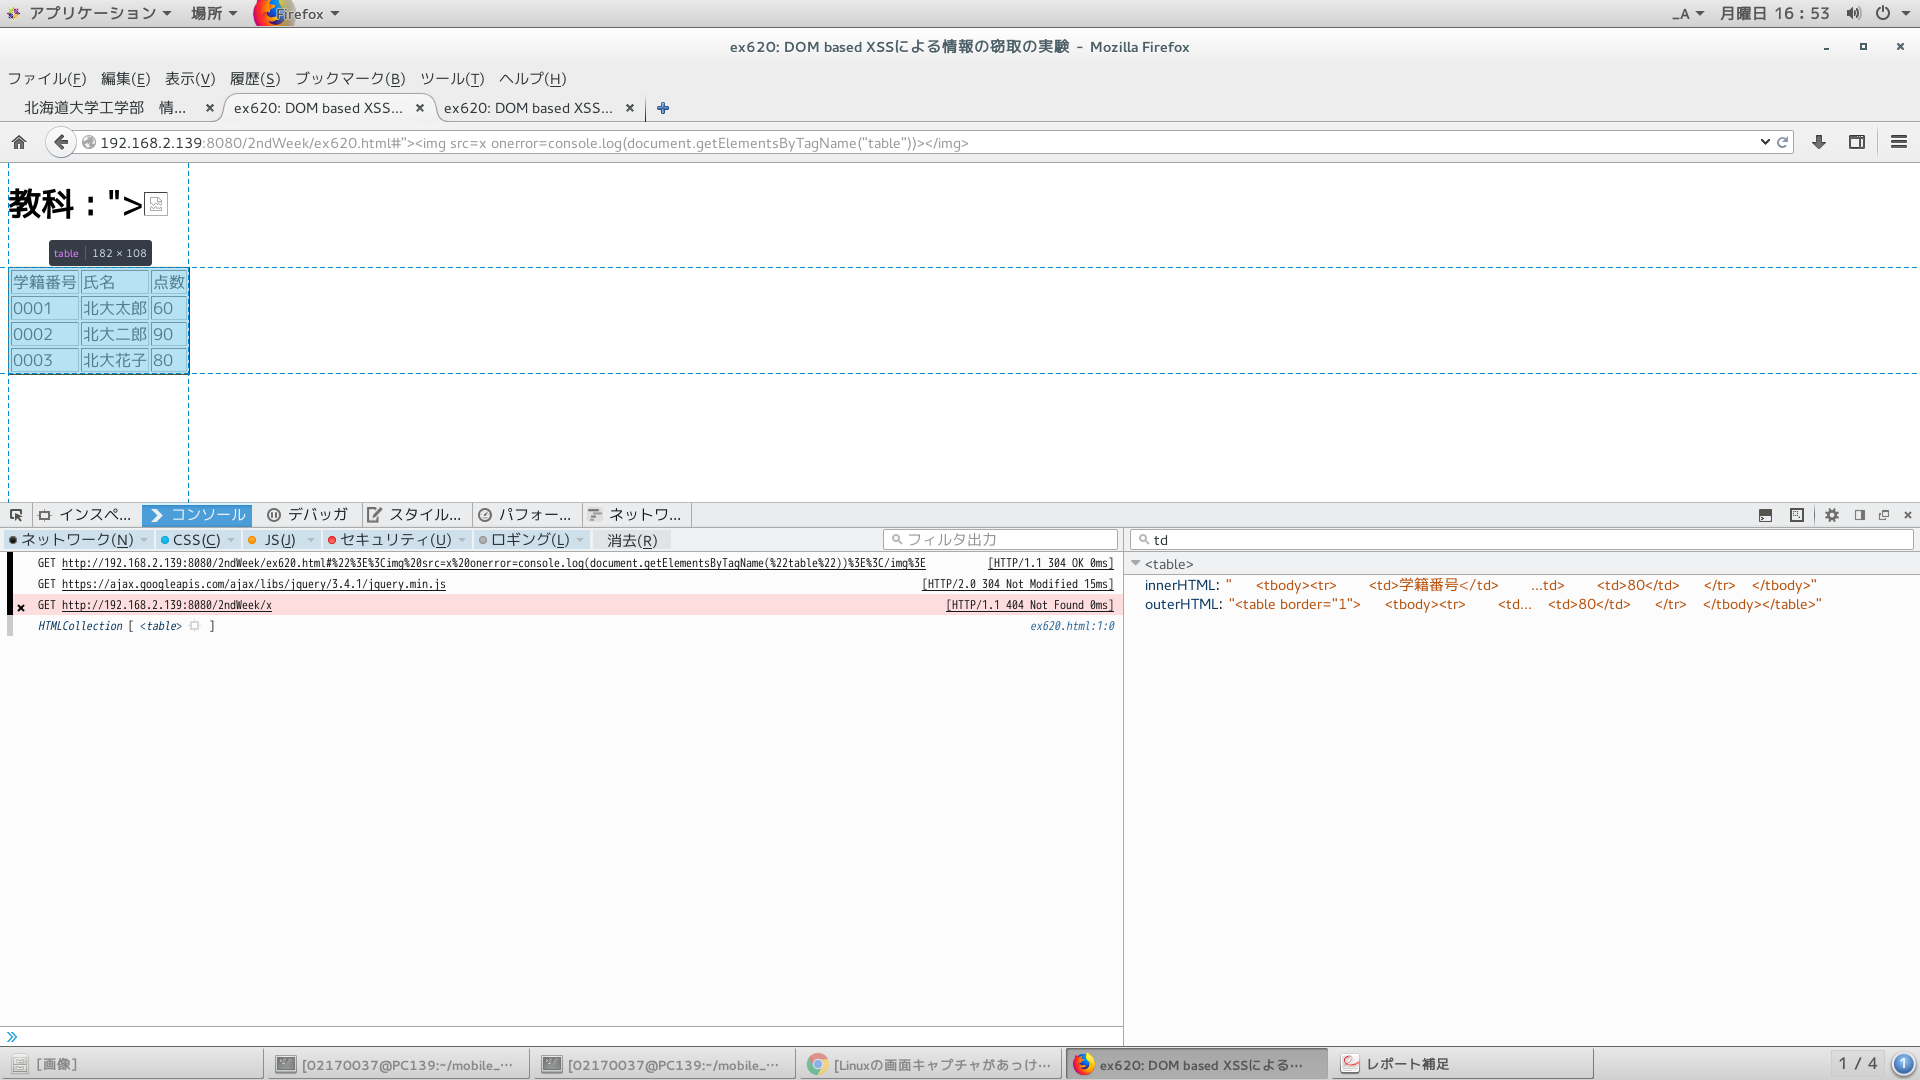
\includegraphics[width=13cm]{../webapp/png/6_2_1.png}
    \caption{6\_2\_1.png}
  \end{figure}


  \vspace{1cm}
  \begin{figure}[htbp]
    \centering
    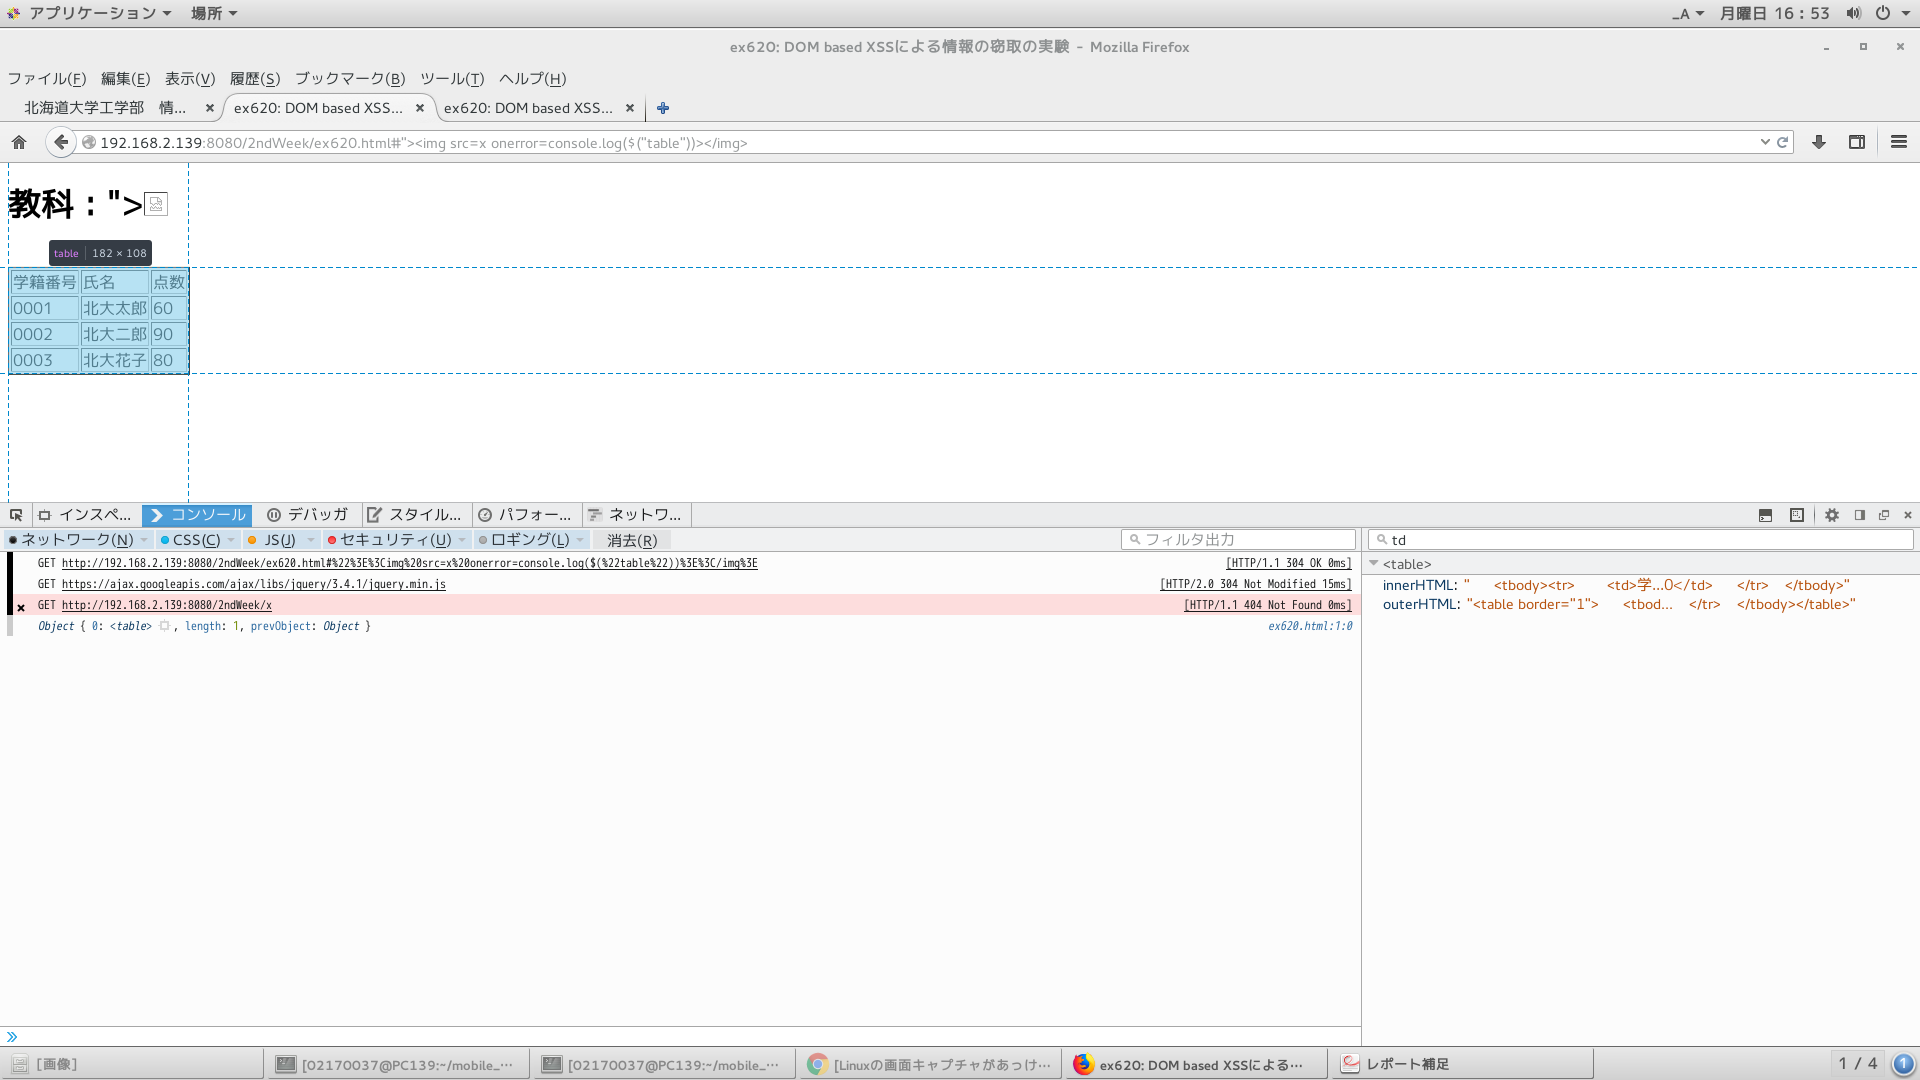
\includegraphics[width=13cm]{../webapp/png/6_2_2.png}
    \caption{6\_2\_2.png}
  \end{figure}



\end{document}
